\documentclass{article}

\usepackage{babel}
\usepackage{blindtext}
\usepackage{caption}
\usepackage{graphicx}

\author{Ee Xuan Tan (4907531) \and Elvira Voorneveld (4930975) \and William Narchi (5046122)}
\date{Group 40}
\title{Computer Graphics Project}

\begin{document}
    \maketitle

    \section{Work Distribution}
    
    \begin{tabular}{ |p{2.5cm}||p{2.5cm}|p{2.5cm}|p{2.5cm}| }
        \hline
        \textbf{Feature} &\textbf{Ee Xuan} &\textbf{Elvira} &\textbf{William}\\
        \hline
        Shading                        &0\%    &100\%  &0\%\\
        Recursion                      &0\%    &0\%    &100\%\\
        Hard Shadows                   &0\%    &100\%  &0\%\\
        Soft Shadows                   &100\%  &0\%    &0\%\\
        BVH                            &40\%   &20\%   &40\%\\
        Interpolation                  &0\%    &100\%  &0\%\\
        Planar Area                    &100\%  &0\%    &0\%\\
        Bloom Filter                   &0\%    &0\%    &100\%\\
        Anti-aliasing                  &0\%    &0\%    &100\%\\
        Several Rays                   &0\%    &0\%    &100\%\\
        \hline
    \end{tabular}

    \section{Features}
    \subsection{Main Requirements}
    \subsubsection{Phong Shading}
    At each intersection point, the diffuse and specular terms from the Phong Model are used to calculate the 
    lighting. We ignore the ambient term, as it is a crude approximation of global illumination, and therefore 
    not necessary to incorporate. First, the lighting is computed separately for every light source in the 
    scene, and those results are then added together to compute the final, direct illumination.

    \begin{center}
        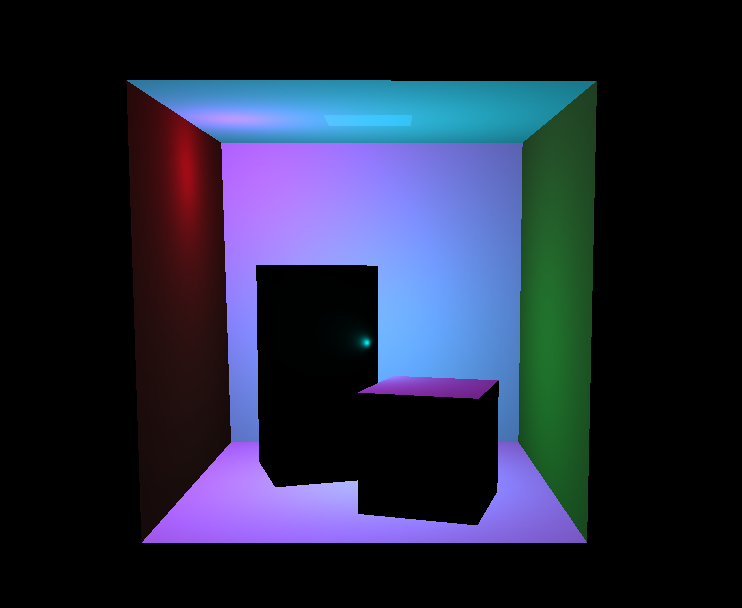
\includegraphics[scale=0.60]{images/phong_shading_showcase}

        The lighting effects produced by phong shading with two light sources RGB(255, 0, 255) and 
        RGB(0, 255, 255)

        \vspace{5mm}

        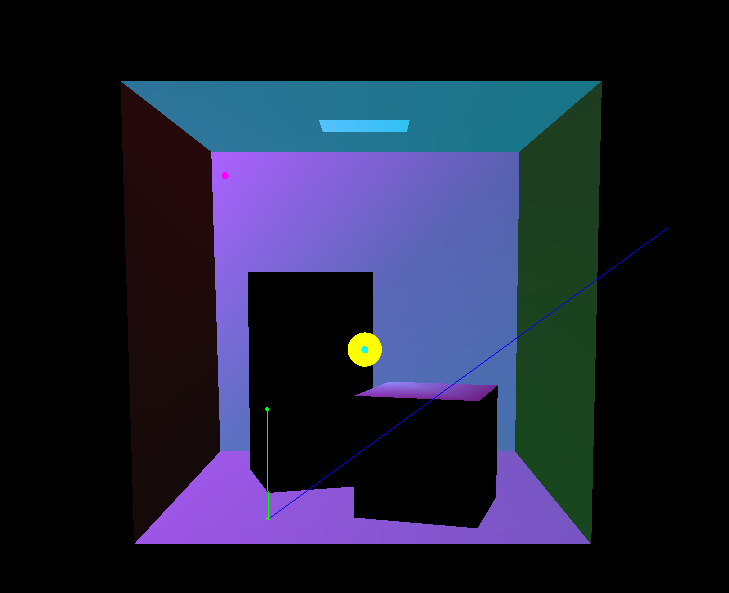
\includegraphics[scale=0.60]{images/phong_shading_debug}

        The phong shading debug, showing one ray shot from another angle, along with its normal
    \end{center}

    \subsubsection{Recursive Ray Tracing}
    The recursive ray tracer builds upon the previously implemented ray shading,
    creating reflection rays at each intersection point and adding the value of the reflection ray's lighting 
    to the initial ray's specular component, provided that the intersection point is on a specular surface 
    and that the reflected ray intersects a surface. This is done recursively until one of the previously 
    mentioned limiting conditions applies or the recursion depth reaches a pre-set \emph{RECURSION\_LIMT}.

    \begin{center}
        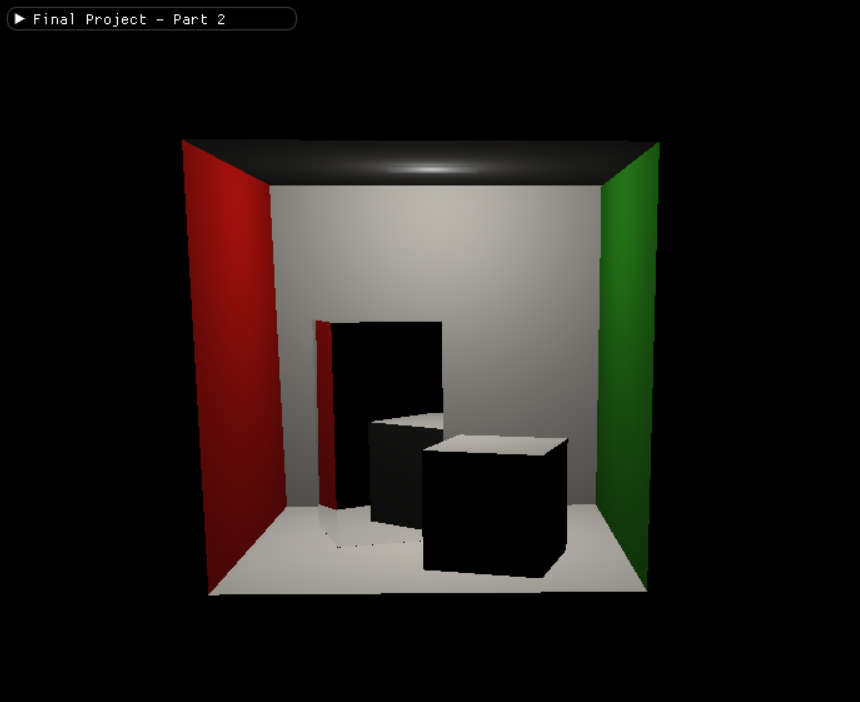
\includegraphics[scale=0.65]{images/recursive_ray_tracer_showcase}

        The complex specular effects produced by recursive ray tracing, which include proper mirror simulation

        \vspace{5mm}

        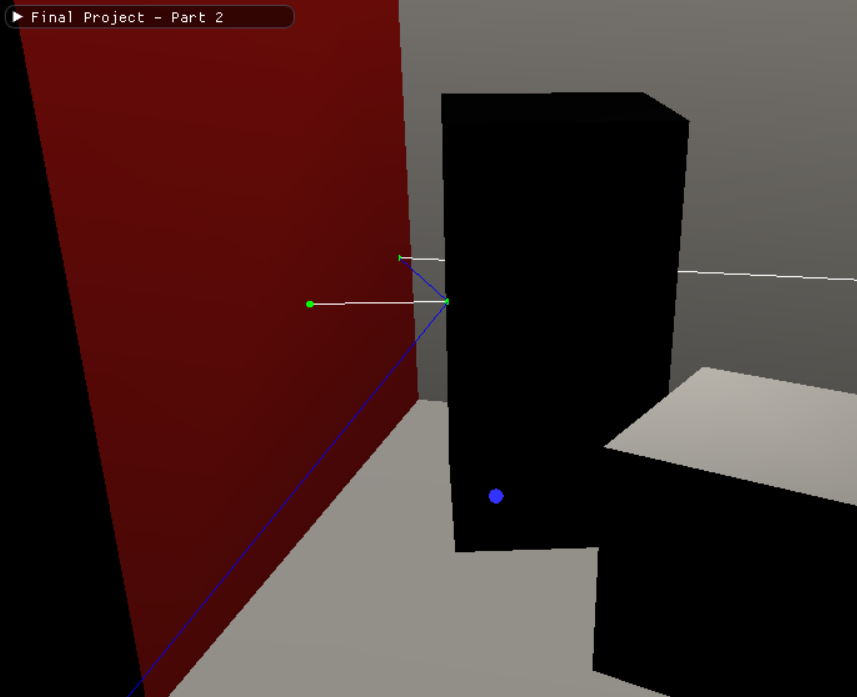
\includegraphics[scale=0.65]{images/recursive_ray_tracer_debug}

        The recursive ray tracer debug, showing two total rays in the recursive chain, along with their normals
    \end{center}

    \subsubsection{Hard Shadows}
    To discover which light source(s) contribute to the lighting of a certain point, ray(s) are shot from the 
    intersection point towards the light source(s). For each light source, it is computed whether or not there 
    is a direct path between the intersection point and the respective light source. Only point lights that 
    directly shine upon the intersection point will be considered when computing the lighting in that area,
    leaving it black if none of the point lights contribute.

    \begin{center}
        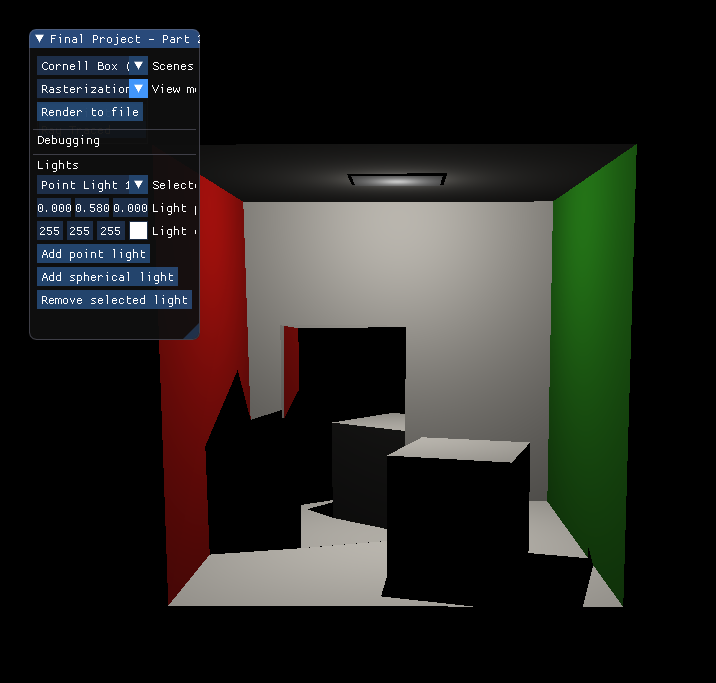
\includegraphics[scale=0.60]{images/hard_shadow_showcase}

        The result of using a single point light source to create hard shadows.

        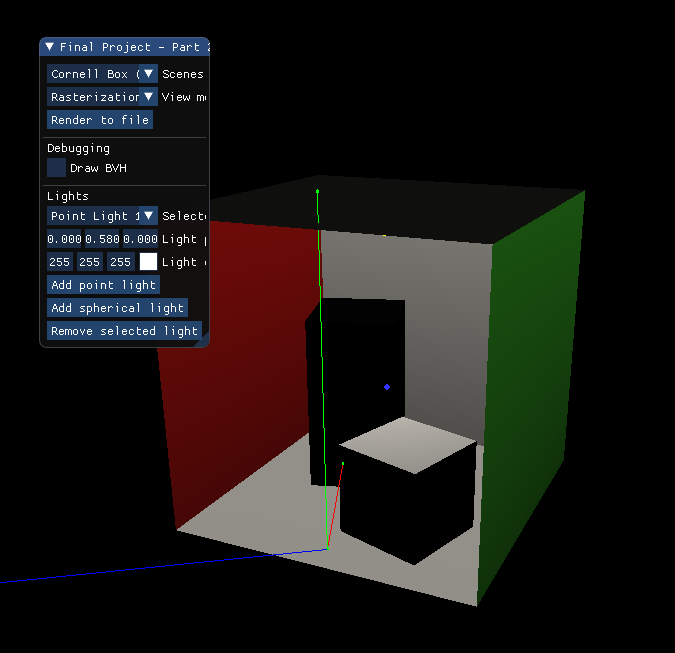
\includegraphics[scale=0.65]{images/hard_shadow_debug}

        The hard shadow debug, showing a ray shot from another angle, along with its normal and a red line 
        indicating the intersection with another object before reaching the point light source.
    \end{center}

    \subsubsection{Soft Shadows}
    The first step to the implementing the soft shadows is to generate uniformly distributed rays from the 
    spherical light source. In order, to get a uniform distribution of rays from the lightsource, the idea of 
    the fibonacci sequence was used, by generating unifromly distributed step sizes using the golden ratio. 
    The second problem, was to remove light rays from the 'wrong' side of the light source, this was done by 
    using the center of the sphere and radius to calculate the longest the light ray on the 'right' side could 
    be. So, by using this method we are able to check each randomly generated sample of the light. Finally, a 
    number of sample points are taken, from these sample points we check to see if they are on the 'right' 
    side of the sphere and if the sample ray does not intersect an object. For each point we then divide the 
    lighting value obtained by the number of sample rays taken from the sphere, giving the average light value. 

    \begin{center}
        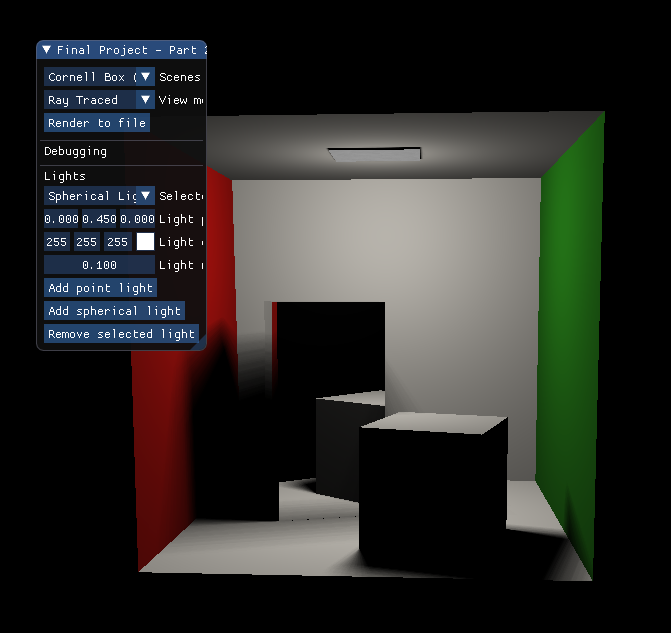
\includegraphics[scale=0.80]{images/soft_shadow_showcase}

        The result of using a single spherical light source with the \emph{SPHERE\_SAMPLE\_LIMIT} set to 100 
        to create soft shadows.

        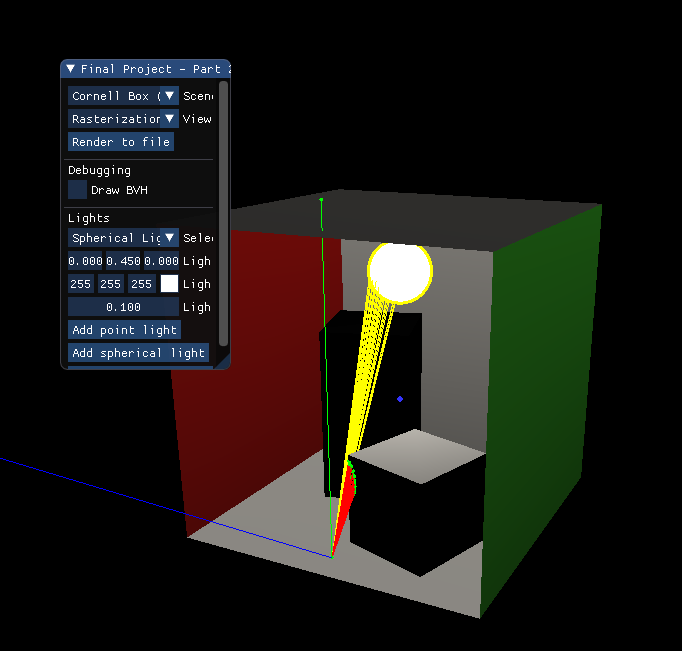
\includegraphics[scale=0.80]{images/soft_shadow_debug}

        The soft shadow debug, showing all of the uniformly distributed samples generated by the spherical 
        light source. The yellow lines indicate a direct path from the intersection to the light source and 
        the red lines indicate the intersection with another object before reaching the spherical light source.
    \end{center}

    \subsubsection{Bounding Volume Hierarchy}
    This Bounding Volume Hierarchy (BVH) is contructed using the Surface Area Heuristic (SAH) and binning. 
    It starts off by indexing every triangle in the model and creating the first Axis-Aligned Bounding Box 
    (AABB) that contains all of the triangles. It then proceeds to split this bounding box until the maximum 
    level or the minimum amount of triangles is reached. Splitting relies on the use of alternating axes and 
    bins to create a split boundary. It goes on to compute the cost function of these new splits, and only 
    creates new nodes for them if they are more efficient to use than the original. After constructing the 
    BVH, it will recursively check if a ray shot at the scene will intersect with the parent AABB or any of 
    its children. If there is no intersection with any of the leaf nodes, there is no intersection with the 
    model. Otherwise, all triangles in the respective leaf node will be checked for intersection.
    Two constructors are provided for the BVH: one where the maximum tree depth can be manually set;
    and one where the number of triangles in the scene is used as a heuristic to determine the maximum
    tree depth.

    \begin{figure}[!htb]
        \minipage{0.49\textwidth}
          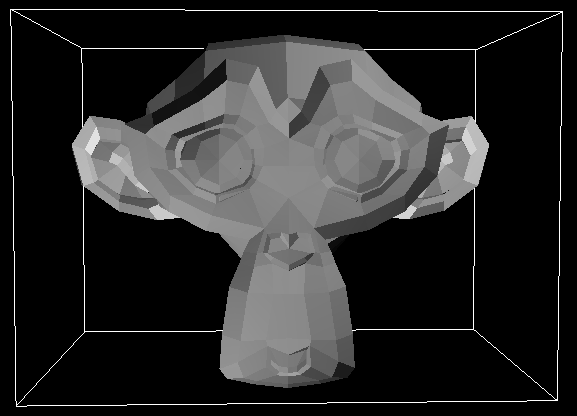
\includegraphics[width=\linewidth, height=5cm]{images/bvh_level_one}
          \caption*{The first level of the BVH}
        \endminipage\hfill
        \minipage{0.49\textwidth}
          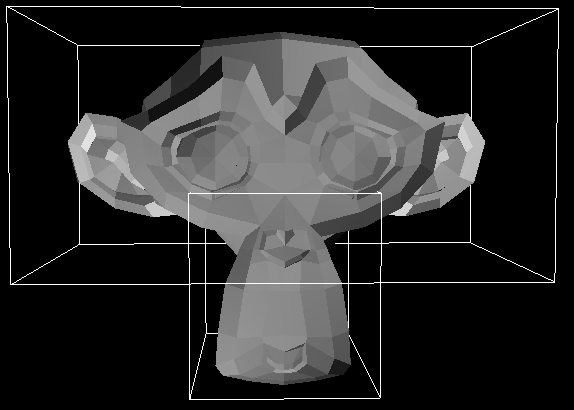
\includegraphics[width=\linewidth, height=5cm]{images/bvh_level_two}
          \caption*{The second level of the BVH}
        \endminipage
        \newline
        \minipage{0.49\textwidth}
          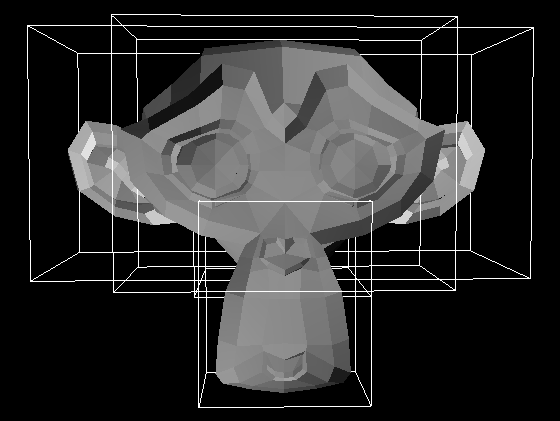
\includegraphics[width=\linewidth, height=5cm]{images/bvh_level_three}
          \caption*{The third level of the BVH}
        \endminipage\hfill
        \minipage{0.49\textwidth}
          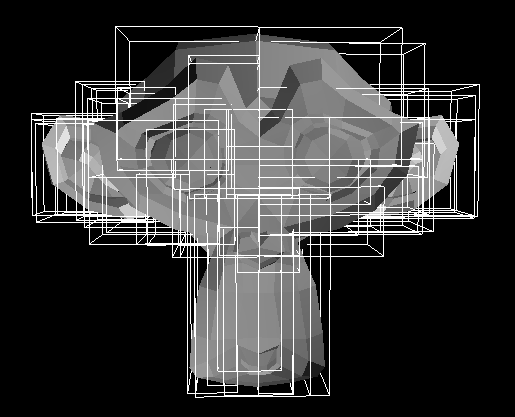
\includegraphics[width=\linewidth, height=5cm]{images/bvh_level_ten}
          \caption*{The tenth level of the BVH}
        \endminipage
    \end{figure}

    \subsection{Extra Requirements}
    \subsubsection{Interpolation}
    To be constructed

    \subsubsection{Planar Area Light}
    To be constructed

    \subsubsection{Bloom Filter}
    A simple bloom filter that uses a box blur filter for the underlying blurring. It functions very similarly 
    to what was described in the slides for lecture 3, in that it culls pixels below a particular threshold 
    and applies the box filter implementation described in the slides onto the filtered pixels, before adding 
    the result to the un-processed pixel values. Due to the flatness of the available scenes' colour range,
    the bloom filter looks slightly exaggerated.

    \begin{figure}[!htb]
        \minipage{0.49\textwidth}
          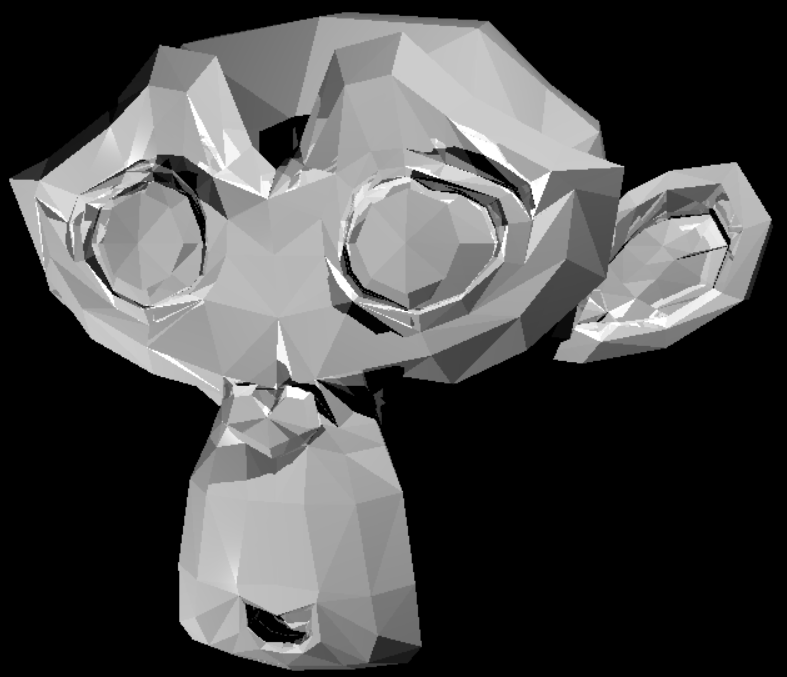
\includegraphics[width=\linewidth, height=6cm]{images/monkey_no_bloom}
          \caption*{Monkey without bloom}
        \endminipage\hfill
        \minipage{0.49\textwidth}
          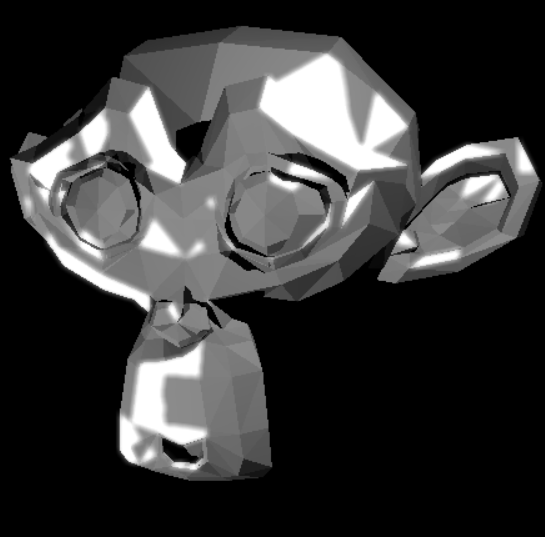
\includegraphics[width=\linewidth, height=6cm]{images/monkey_bloom}
          \caption*{Monkey with bloom}
        \endminipage
    \end{figure}
    
    \subsubsection{Cast Multiple Rays Per Pixel / Anti-Aliasing}
    A simple super-sampling anti-aliasing method that renders multiple rays per pixel (in effect, rendering at a higher resolution) using a uniform distribution of samples.
    The colour values of the sample rays are then averaged with no weighting to produce the final colour value.
    The exact degree of super-sampling can be adjusted via the \emph{SAMPLING\_FACTOR} variable.

    \begin{center}
        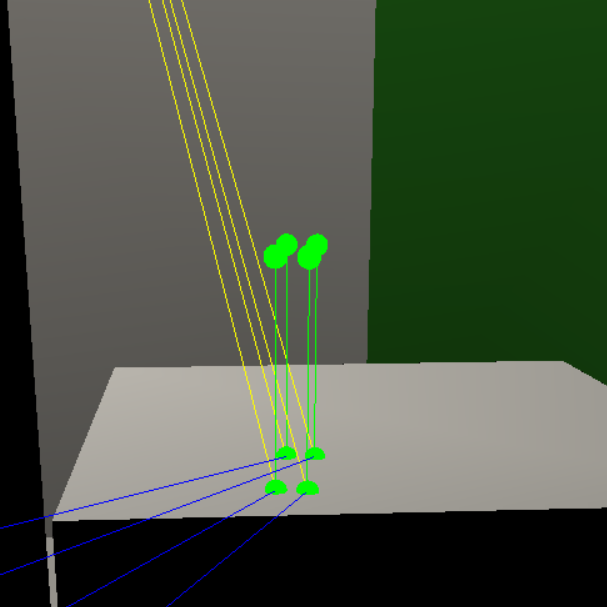
\includegraphics[scale=0.75]{images/supersampling_debugger.png}

        {\footnotesize Visual debug at a 2x super-sampling ratio showing 4 rays in total
        
        (rays are projected from a far distance for easier demonstration)\par}
    \end{center}

    As can be clearly seen, the end result is a much smoother image,
    with far fewer visible jagged edges and higher overall fidelity.

    \begin{figure}[!htb]
        \minipage{0.49\textwidth}
          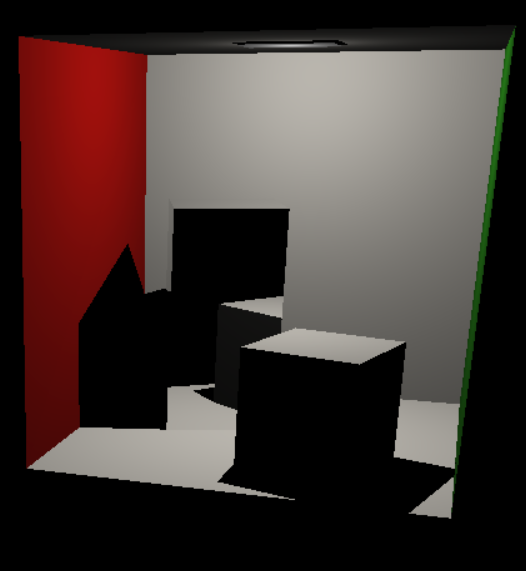
\includegraphics[width=\linewidth, height=6cm]{images/supersampling_non_supersampled}
          \caption*{Render without super-sampling}
        \endminipage\hfill
        \minipage{0.49\textwidth}
          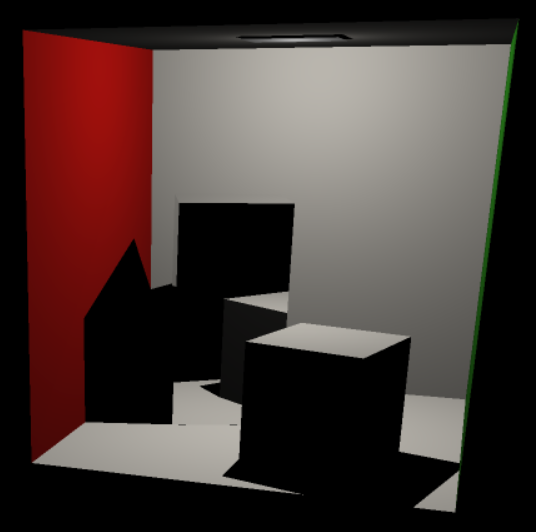
\includegraphics[width=\linewidth, height=6cm]{images/supersampling_supersampled}
          \caption*{Render with 2x super-sampling}
        \endminipage
    \end{figure}

    \section{Models}
    To be constructed

    \section{Performance Test}
    To be constructed
\end{document}
